\documentclass[border=4pt]{standalone}
\usepackage{amsmath,amssymb}
\usepackage{tikz}
\usetikzlibrary{arrows.meta}
\begin{document}
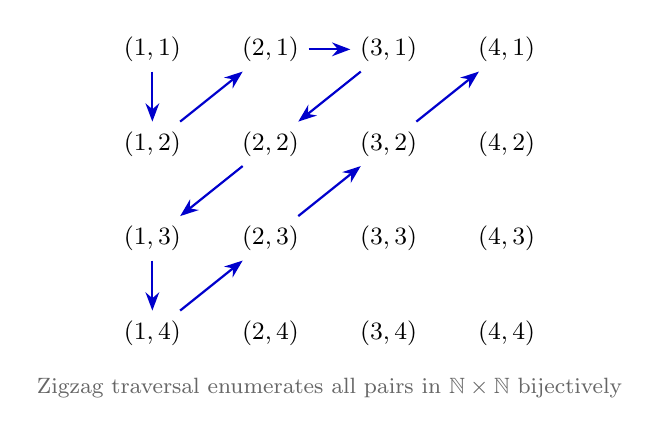
\begin{tikzpicture}[font=\small, >=Stealth]
  \foreach \x in {1,2,3,4} {
    \foreach \y in {1,2,3,4} {
      \node (p\x\y) at (\x*1.5, -\y*1.2) {$(\x,\y)$};
    }
  }
  % Draw arrows
  \draw[->, thick, blue!80!black] (p11) -- (p12);
  \draw[->, thick, blue!80!black] (p12) -- (p21);
  \draw[->, thick, blue!80!black] (p21) -- (p31);
  \draw[->, thick, blue!80!black] (p31) -- (p22);
  \draw[->, thick, blue!80!black] (p22) -- (p13);
  \draw[->, thick, blue!80!black] (p13) -- (p14);
  \draw[->, thick, blue!80!black] (p14) -- (p23);
  \draw[->, thick, blue!80!black] (p23) -- (p32);
  \draw[->, thick, blue!80!black] (p32) -- (p41);
  
  \node[font=\footnotesize, text=gray!80!black, align=center] at (3.75, -5.5) 
    {Zigzag traversal enumerates all pairs in $\mathbb{N} \times \mathbb{N}$ bijectively};
\end{tikzpicture}
\end{document}